\documentclass[10pt]{beamer}	% Is better for some Windows user.
%
\usepackage{pict2e}
\usepackage{tikz}
\usepackage[english]{babel} % Pakete laden
\usepackage[utf8]{inputenc}
\usepackage[T1]{fontenc}
\usepackage{graphicx, xcolor}
% \usepackage{BeamerColor}
\usepackage{tikz, amsfonts, amsmath}
\usetheme{Goettingen}
% \usecolortheme[named=darkgray]{structure}
\def\UDM{ % untere Dreiecks-Matrix
\mbox{
\setlength{\unitlength}{9pt}
\begin{picture}(1,1)
\put(0,1){\line(1,0){1}}
\put(1,0){\line(0,1){1}}
\put(0,1){\line(1,-1){1}}
\end{picture}
}}
\title{Extended Finite Element Method (XFEM)}
\author{Janna Puderbach}
% \input{docinfo}				% Edit here author informations.
% \input{header}
% \input{titlepage}
% \input{headingsandfooter}
\usepackage{algorithm2e}
\begin{document}
    \addtocounter{framenumber}{-1}	% Exclude page from pagecounter.
   	\begin{frame}[plain]
		\titlepage
	\end{frame}
	%
	%\setcounter{framenumber}{0}
	\frame{
		\frametitle{Content}
		\tableofcontents
	} 

\section{Motivation}

\begin{frame}{Motivation}
    \begin{figure}
        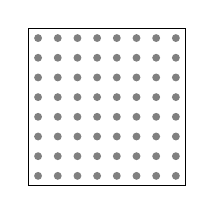
\begin{tikzpicture}
            %microscopic structure
            \draw (-1,-1) -- (-1,1) -- (1,1) -- (1,-1) -- (-1,-1);

            \foreach \x in {1,...,8}
            {
                \foreach \y in {1,...,8}
                {
                    \fill[gray] (-1.125 + \x/4,-1.125 + \y/4) circle (0.5mm);
                }
            }
    
        \end{tikzpicture}
        \caption{Microstructure of a composite material}
    \end{figure}
	Applications:
	\begin{itemize}
        \item Crack propagation
        \item Microstructured problems
        \item Composite materials
        \item Time-depending domains
	\end{itemize}
    Advantages:
    \begin{itemize}
        \item Discontinuities within elements possible
        \item Avoiding complex mesh generation
    \end{itemize}
\end{frame}
	
\section{Interface Problems}
\begin{frame}{Interface Problems}
	\begin{figure}
        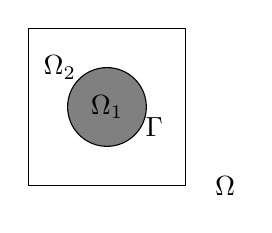
\begin{tikzpicture}

        % composite material
            \draw (4.25,0.25) -- (4.25,2.25) -- (6.25,2.25) -- (6.25,0.25) -- (4.25,0.25);
            \fill[gray] (5.25,1.25) circle (5mm);
            \draw  (5.25,1.25) circle (5mm);
            \node at (4.65,1.75) {$\Omega_2$};
            \node at (5.25,1.25) {$\Omega_1$};
            \node at (6.75,0.25) {$\Omega$};
            \node at (5.85,1) {$\Gamma$};
        \end{tikzpicture}
        \caption{Composite material}
        \label{fig:composite_material}
    \end{figure}
    \begin{align}
        - \nabla \cdot (\mu_i \nabla u_i) &= f & \text{ in } \Omega_i \\
        u_i&= g& \text{ on } \partial \Omega \\
        [u]& = g_s& \text{ on } \Gamma
    \end{align}
\end{frame}
\section{Unfitted Method}
\begin{frame}{Unfitted Method}
	
	\begin{itemize}
        \item background mesh
        \item cut cells
    \end{itemize}
	
	\begin{figure}
        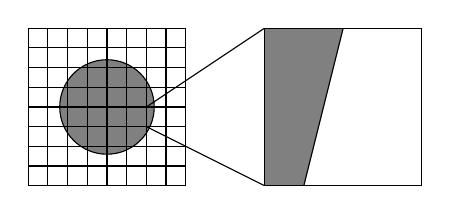
\begin{tikzpicture}
	
            \fill[gray] (0,0) circle (6mm);
            \draw  (0,0) circle (6mm);
	
            \foreach \x in {0,...,8}
            {
                \draw (-1 + \x/4, -1) -- (-1 + \x/4, 1);
            }
            \foreach \x in {0,...,8}
            {
                \draw (-1,-1 + \x/4) -- (1,-1 + \x/4);
            }
            \fill[gray] (2,-1) -- (2.5,-1) -- (3,1) -- (2,1) -- (2,-1);
            \draw (2,-1) -- (4,-1) -- (4,1) -- (2,1) -- (2,-1);
            \draw (0.5,0) -- (2,1);
            \draw (0.5,-0.25) -- (2,-1);
            \draw (2.5,-1) -- (3,1);
        \end{tikzpicture}
        \caption{Unfitted mesh}
    \end{figure}
	
	% Complex microstructure
	% Level set
	% Difference to cut cell?	
\end{frame}

\section{Level Set Function}
\begin{frame}{Level Set Function}
	\begin{itemize}
        \item Tracking the interface
	\end{itemize}
	\begin{align*}
        \phi : \Omega \to \mathbb{R} \quad , \quad
        \phi(x) \begin{cases}
        = 0 & , x \in \Gamma\\
        < 0 &, x \in  \Omega_1\\
        > 0 &, x \in  \Omega_2
        \end{cases}
	\end{align*}
	
    \begin{figure}
        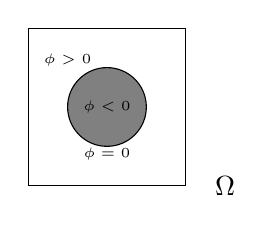
\begin{tikzpicture}

        % composite material
            \draw (4.25,0.25) -- (4.25,2.25) -- (6.25,2.25) -- (6.25,0.25) -- (4.25,0.25);
            \fill[gray] (5.25,1.25) circle (5mm);
            \draw  (5.25,1.25) circle (5mm);
            \node at (4.75,1.85) {\tiny{$\phi > 0$}};
            \node at (5.25,1.25) {\tiny{$\phi < 0$}};
            \node at (5.25,0.65) {\tiny{$\phi = 0$}};
            \node at (6.75,0.25) {$\Omega$};
	
        \end{tikzpicture}
        \caption{Level set function}
        \label{fig:level_set}
    \end{figure}
    
    \begin{itemize}
        \item i.e. signed distance function
    \end{itemize}
	
\end{frame}

\begin{frame}{Implementation in deal.II}
    \begin{figure}
        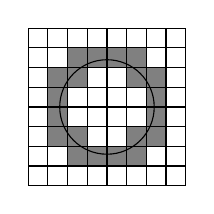
\begin{tikzpicture}

            \fill[gray] (-0.5,0.5) rectangle (0.5,0.75);
            \fill[gray] (-0.5,-0.5) rectangle (0.5,-0.75);
            \fill[gray] (-0.75,-0.5) rectangle (-0.5,0.5);
            \fill[gray] (0.75,-0.5) rectangle (0.5,0.5);
            \fill[gray] (-0.5,0.25) rectangle (-0.25,0.5);
            \fill[gray] (0.5,0.25) rectangle (0.25,0.5);
            \fill[gray] (-0.5,-0.25) rectangle (-0.25,-0.5);
            \fill[gray] (0.5,-0.25) rectangle (0.25,-0.5);

            \draw  (0,0) circle (6mm);
            \foreach \x in {0,...,8}
            {
                \draw (-1 + \x/4, -1) -- (-1 + \x/4, 1);
            }
                \foreach \x in {0,...,8}
            {
                \draw (-1,-1 + \x/4) -- (1,-1 + \x/4);
            }
        \end{tikzpicture}
        \caption{Cut cells}
    \end{figure}

    \begin{itemize}
        \item loop over all cells
        \item using the level set function to find the cut cells
        \item \texttt{active\_fe\_index()}
    \end{itemize}
    % strong code
    % fe systems
    % Fe collection
    % xfe_values
\end{frame}

\section{Extended Finite Elements}


\begin{frame}{Enriched Elements}
    \only <1->
    {\begin{figure}
        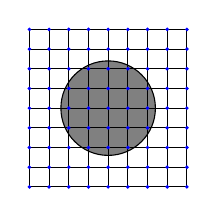
\begin{tikzpicture}
	
            \fill[gray] (0,0) circle (6mm);
            \draw  (0,0) circle (6mm);
	
            \foreach \x in {0,...,8}
            {
                \draw (-1 + \x/4, -1) -- (-1 + \x/4, 1);
            }
            \foreach \x in {0,...,8}
            {
                \draw (-1,-1 + \x/4) -- (1,-1 + \x/4);
            }
    
            \foreach \x in {0,...,8}
            {
                \foreach \y in {0,...,8}
                {
                    \filldraw[blue] (-1 +\x/4,-1 + \y/4) circle (0.15mm);
                }
            }
%             \foreach \x in {0,...,4}
%             {
%                 \draw[thin,red] (-0.5 + \x/4,0.75) circle (0.5mm);
%                 \draw[thin,red] (-0.5 + \x/4,-0.75) circle (0.5mm);
%             }
%             \foreach \x in {0,...,6}
%             {
%                 \draw[thin,red] (-0.75 + \x/4,0.5) circle (0.5mm);
%                 \draw[thin,red] (-0.75 + \x/4,-0.5) circle (0.5mm);
%             }
%             \foreach \x in {0,...,2}
%             {
%                 \draw[thin,red] (-0.75 + \x/4,0.25) circle (0.5mm);
%                 \draw[thin,red] (-0.75 + \x/4,-0.25) circle (0.5mm);
%                 \draw[thin,red] (0.25 + \x/4,0.25) circle (0.5mm);
%                 \draw[thin,red] (0.25 + \x/4,-0.25) circle (0.5mm);
%             }
%             \foreach \x in {0,1}
%             {
%                 \draw[thin,red] (-0.75 + \x/4,0) circle (0.5mm);
%                 \draw[thin,red] (0.5 + \x/4,0) circle (0.5mm);
%             }
        \end{tikzpicture}
        \caption{Standard degrees of freedom}
%     \end{figure}}
    
% \only <2>
%     {\begin{figure}
        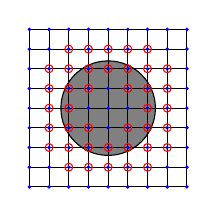
\begin{tikzpicture}
	
            \fill[gray] (0,0) circle (6mm);
            \draw  (0,0) circle (6mm);
	
            \foreach \x in {0,...,8}
            {
                \draw (-1 + \x/4, -1) -- (-1 + \x/4, 1);
            }
            \foreach \x in {0,...,8}
            {
                \draw (-1,-1 + \x/4) -- (1,-1 + \x/4);
            }
    
            \foreach \x in {0,...,8}
            {
                \foreach \y in {0,...,8}
                {
                    \filldraw[blue] (-1 +\x/4,-1 + \y/4) circle (0.15mm);
                }
            }
            \foreach \x in {0,...,4}
            {
                \draw[thin,red] (-0.5 + \x/4,0.75) circle (0.5mm);
                \draw[thin,red] (-0.5 + \x/4,-0.75) circle (0.5mm);
            }
            \foreach \x in {0,...,6}
            {
                \draw[thin,red] (-0.75 + \x/4,0.5) circle (0.5mm);
                \draw[thin,red] (-0.75 + \x/4,-0.5) circle (0.5mm);
            }
            \foreach \x in {0,...,2}
            {
                \draw[thin,red] (-0.75 + \x/4,0.25) circle (0.5mm);
                \draw[thin,red] (-0.75 + \x/4,-0.25) circle (0.5mm);
                \draw[thin,red] (0.25 + \x/4,0.25) circle (0.5mm);
                \draw[thin,red] (0.25 + \x/4,-0.25) circle (0.5mm);
            }
            \foreach \x in {0,1}
            {
                \draw[thin,red] (-0.75 + \x/4,0) circle (0.5mm);
                \draw[thin,red] (0.5 + \x/4,0) circle (0.5mm);
            }
        \end{tikzpicture}
        \caption{Enriched degrees of freedom}
    \end{figure}}    

\end{frame}


\begin{frame}{Standard Finite Elements}
    \begin{itemize}
         \item Standard finite element space
         \begin{align*}
            V_h = \left\{ \varphi \in V : \phi|_K \in Q_p \right\}
         \end{align*}
         \item Enriched finite element space
         \begin{align*}
            V_h^s = \left\{ \varphi \in V : \varphi|_K \in Q , \varphi|_{K_i} \in Q, i=1,2\right\}
         \end{align*}
    \end{itemize}
\end{frame}


\begin{frame}{Finite Element Solution}
    \begin{itemize}
    \item Standard finite Element solution
    \begin{align}
        u_h = \sum_{i \in I} u_i N_i
    \end{align}
    where $N_i$ are standard shape functions.


    \item Extended finite element solution
    \begin{align}
        u_h = \sum_{i \in I} u_i N_i + \sum_{j \in J} a_j M_j
    \end{align}
    where $M_j$ are enriched shape functions.
    \begin{align}
    M_j(x) = N_j(x) \Psi(x)
    \end{align}
    with $\Psi$ the Heaviside function.
    \end{itemize}
%
%     % Shape functions
%     % picture
%     % standard functions
\end{frame}
    
% \begin{frame}{Boundary and Interface condition}
%     %
% \end{frame}
%
% \begin{frame}{Implementation in deal.II}
%     \begin{figure}
%         \begin{tikzpicture}
%
%             \fill[gray] (-0.5,0.5) rectangle (0.5,0.75);
%             \fill[gray] (-0.5,-0.5) rectangle (0.5,-0.75);
%             \fill[gray] (-0.75,-0.5) rectangle (-0.5,0.5);
%             \fill[gray] (0.75,-0.5) rectangle (0.5,0.5);
%             \fill[gray] (-0.5,0.25) rectangle (-0.25,0.5);
%             \fill[gray] (0.5,0.25) rectangle (0.25,0.5);
%             \fill[gray] (-0.5,-0.25) rectangle (-0.25,-0.5);
%             \fill[gray] (0.5,-0.25) rectangle (0.25,-0.5);
%
%             \draw  (0,0) circle (6mm);
%             \foreach \x in {0,...,8}
%             {
%                 \draw (-1 + \x/4, -1) -- (-1 + \x/4, 1);
%             }
%                 \foreach \x in {0,...,8}
%             {
%                 \draw (-1,-1 + \x/4) -- (1,-1 + \x/4);
%             }
%         \end{tikzpicture}
%         \caption{Cut cells}
%     \end{figure}
%
%     \begin{itemize}
%         \item loop over all cells
%         \item using the level set function to find the cut cells
%         \item \texttt{active\_fe\_index()}
%     \end{itemize}
%     % strong code
%     % fe systems
%     % Fe collection
%     % xfe_values
% \end{frame}
%
% \begin{frame}{XFEValues Class}
%     % quadrature
%     % cubelements
%     % Interface condition
% \end{frame}
    
\end{document}
